\documentclass[]{article}
\addtolength{\oddsidemargin}{-.875in}
\addtolength{\evensidemargin}{-.875in}
\addtolength{\textwidth}{1.75in}

\addtolength{\topmargin}{-.875in}
\addtolength{\textheight}{1.75in}

\usepackage{graphicx}
%opening
\title{LiRX V2}
\author{}
\date{}

\begin{document}

\maketitle

\begin{abstract}
	LiRX - Licht Receiver.
	
		
	
	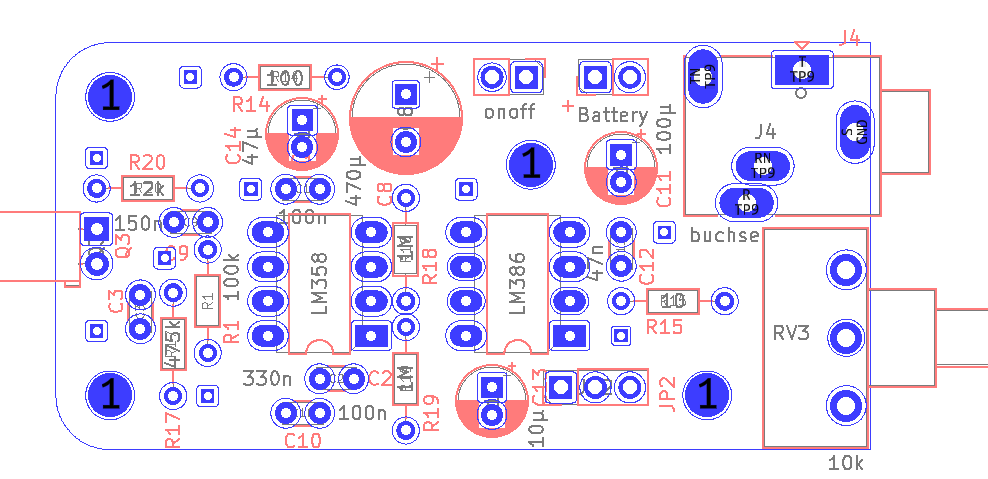
\includegraphics[width=1.0\linewidth]{Platine.png}

\end{abstract}

\section{Bauteile}
Liste der elektronischen Bauteile in aufsteigender Bauhöhe.
\subsection{Widerstände}
Empfohlene Werte für die Widerstände:
\begin{itemize}
	\item R1 :	100k$\Omega$ - Forward Widerstand 
	\item R2 :  680$\Omega$ - Begrenzung Lautstärke \#1
	\item R3 : 	270$\Omega$ - Begrenzung Lautstärler \#2
	\item R14 : 100$\Omega$ - Entkopplung LM358 Stromversorgung
	\item R15 : 10$\Omega$ - optional - Endfilter LM386
	\item R17 : 470k$\Omega$ - Feedback Widerstand
	\item R18 : 12k$\Omega$ - Für Spannungsteiler virtual GND 
	\item R19 : 12k$\Omega$ - Für Spannungsteiler virtual GND
	\item R20 : 12k$\Omega$ - Strom für Photosensor
\end{itemize}
\subsection{Fassungen und Buchse}
\begin{itemize}
	\item 8pol Fassung für LM358, Dual Operationsverstärker
	\item 8pol Fassung für LM386, Mono Audioverstärker
	\item 3,5mm Klinkenbuchse
\end{itemize}
\subsection{Kerko Kondensatoren}
\begin{itemize}
	\item C1 : 100nF - Spannungsstabilisation
	\item C2 : 100nF - Spannungsstabilisation
	\item C3 : 18pf - optional - um hochfrequente Verstärkung des LM358 zu verringern
	\item C9 : 150nF - Gleichspannung auskoppeln
	\item C10 : 330nF - Gleichspannung auskoppeln
	\item C12 : 47nF - Endfilter LM386	
\end{itemize}
\subsection{Elko Kondensatoren}
Auf Polung achten!
\begin{itemize}
	\item C8: 470$\mu$F $\oslash$8mm - Spannungsstabilisation
	\item C11: 100$\mu$F $\oslash$5mm - Entkopplung Audiosignal Gleichstrom
	\item C13: 10$\mu$F $\oslash$5mm - optional - Verstärkungsboost LM386
	\item C14: 47$\mu$F  $\oslash$5mm - Spannungsstabilisation
\end{itemize}
\subsection{Photosensor}
Wahlweise Photodiode oder Phototransistor.

Auf Polung achten, sonst funktioniert es nicht.

Alternativ kann auch jede Leuchtdiode als Photosensor ausgetestet werden. Ein Photowiderstand wird jedoch zu träge sein.
\subsection{Schalter}]
Für den LM386 ist ein Schalter "gain" vorgesehen, um die Verstärkung des LM386 zu vergrößern.

Für die Stromversorgung ist ein Schalter "onff" vorgesehen.

\subsection{Stromversorgung}
Es gibt einen Anschluss für eine 9V Batterie. Auf Polung achten!

\subsection{Letzte Komponenten}
Es sind zwei Potentiometerbauformen möglich, nur eines der beiden ist zu verwenden: RV1 oder RV3, ein 10k$\Omega$ Potentiometer.

\section{Notizen zum Schaltplan}
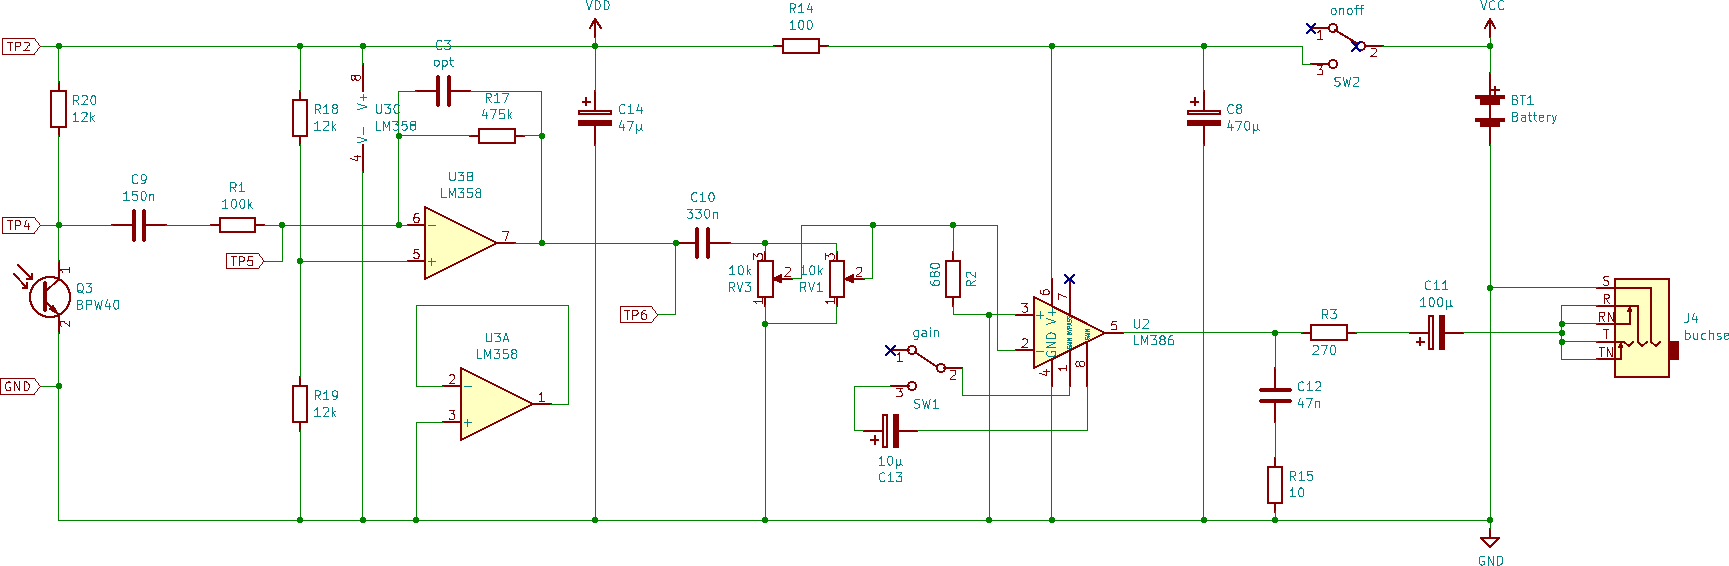
\includegraphics[width=1.0\linewidth]{Schaltplan.png}

Die Schaltung wird mit 9V versorgt.

Der LM386 wird direkt von den 9V gespeist, die Stromversorgung des LM358 wird über R14 entkoppelt.

Von den beiden Operationsverstärkern im LM358 wird nur einer verwendet, der andere ist stillgelegt.

Über R20 wird eine Spannung an Q3, der Photodiode, angelegt. Je nach Menge des einfallenden Lichts leitet die Photodiode mehr oder weniger, weswegen die Spannung vor C9 sich variiert. 

Die beiden Widerstände R18 und R19 dienen als Spannungsteiler und liefern einen "virtuellen Ground" für den Operationsverstärker.

Der Operationsverstärker ist als "invertierender Verstärker" beschaltet, die Verstärkung entspricht $-R17/R1$, als fast das fünffache.

Der optionale Kondensator C3 bildet zusammen mit R17 einen Tiefpass, wodurch hochfrequente Signale weniger stark verstärkt werden. Bei einer Verwendung von C=18pF und R=470k$\Omega$ ist die Grenzfrequenz $F_{3db}=\frac{1}{2 \pi C R}$ ungefähr 18kHz, also schon im nicht mehr hörbaren bereich.

Sowohl C9, C10 als auch C11 sind Gleichspannungsentkopplungen, die den Gleichstromanteil aus den Signalen blockieren.

Das Poti stellt einen Spannungsteiler dar, um die Signalstärker nach dem Operationsverstärker zu reduzieren.

Mit R2 kann man die Signalstärke stärker begrenzen.

Der zuschaltbare Kondensator C13 beim LM386 erlaubt eine Steigerung der Verstärkung des LM386.

C12 und R15 filtern den Ausgang des LM386, wie nach dem Datenblatt.

R3 ist die letzte Lautstärkenbegrenzung und verhindert, dass zu viel Leistung in einen angeschlossenen Kopfhörer geschickt wird.

\section{Abschlussbemerkung}
LiRX ist entstanden auf Impuls von DC3TC.

Diese Platine startete als ein Open Source Nachbau des Empfängers des AATIS Projekt AS802 ``Einfacher Licht-Sende-Empfänger (ELiSE)". Vielen Dank an Aatis!

DC3TC ist auch der Namensgeber für LiRX, den Licht-Receiver. Das Projekt residiert derzeit hier: https://github.com/dk5ee/LiRX.

Weiterer Dank geht an DL3KB, DH5RQ, DL6RBT, DO6RDB, DF1MAT.

\end{document}
